\begin{equation}
    \begin{gathered}
        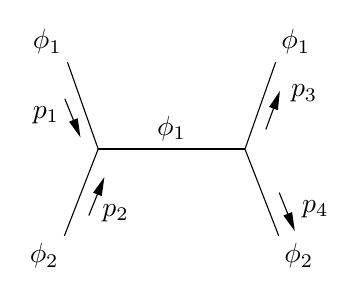
\begin{tikzpicture}[x=0.75pt,y=0.75pt,yscale=-0.75,xscale=0.75]
            %uncomment if require: \path (0,300); %set diagram left start at 0, and has height of 300
            
            %Straight Lines [id:da40464806146453514] 
            \draw    (131.71,79) -- (151.41,134.74) ;
            %Straight Lines [id:da29677111237577014] 
            \draw    (129.71,190.48) -- (151.41,134.74) ;
            %Straight Lines [id:da6874090210216235] 
            \draw    (145.41,177.47) -- (154.66,154.59) ;
            \draw [shift={(155.41,152.74)}, rotate = 472.02] [fill={rgb, 255:red, 0; green, 0; blue, 0 }  ][line width=0.08]  [draw opacity=0] (12,-3) -- (0,0) -- (12,3) -- cycle    ;
            %Straight Lines [id:da30750692746256036] 
            \draw    (130,102.46) -- (139.25,125.33) ;
            \draw [shift={(140,127.18)}, rotate = 247.98000000000002] [fill={rgb, 255:red, 0; green, 0; blue, 0 }  ][line width=0.08]  [draw opacity=0] (12,-3) -- (0,0) -- (12,3) -- cycle    ;
            %Straight Lines [id:da624592681631982] 
            \draw    (151.41,134.74) -- (245.71,134.74) ;
            %Straight Lines [id:da3695208600103763] 
            \draw    (265.41,79) -- (245.71,134.74) ;
            %Straight Lines [id:da5169890936624615] 
            \draw    (267.41,190.48) -- (245.71,134.74) ;
            %Straight Lines [id:da9821639217825291] 
            \draw    (276.96,185.61) -- (267.71,162.74) ;
            \draw [shift={(277.71,187.47)}, rotate = 247.98] [fill={rgb, 255:red, 0; green, 0; blue, 0 }  ][line width=0.08]  [draw opacity=0] (12,-3) -- (0,0) -- (12,3) -- cycle    ;
            %Straight Lines [id:da9298848590018269] 
            \draw    (267.43,99.33) -- (259.12,122.18) ;
            \draw [shift={(268.12,97.46)}, rotate = 110] [fill={rgb, 255:red, 0; green, 0; blue, 0 }  ][line width=0.08]  [draw opacity=0] (12,-3) -- (0,0) -- (12,3) -- cycle    ;
            
            % Text Node
            \draw (129.71,75.6) node [anchor=south east] [inner sep=0.75pt]    {$\phi _{1}$};
            % Text Node
            \draw (127.71,193.88) node [anchor=north east] [inner sep=0.75pt]    {$\phi _{2}$};
            % Text Node
            \draw (128,105.86) node [anchor=north east] [inner sep=0.75pt]    {$p_{1}$};
            % Text Node
            \draw (152.41,168.5) node [anchor=north west][inner sep=0.75pt]    {$p_{2}$};
            % Text Node
            \draw (198.56,131.34) node [anchor=south] [inner sep=0.75pt]    {$\phi _{1}$};
            % Text Node
            \draw (273.62,106.42) node [anchor=south west] [inner sep=0.75pt]    {$p_{3}$};
            % Text Node
            \draw (280.71,173.1) node [anchor=west] [inner sep=0.75pt]    {$p_{4}$};
            % Text Node
            \draw (267.41,75.6) node [anchor=south west] [inner sep=0.75pt]    {$\phi _{1}$};
            % Text Node
            \draw (269.41,193.88) node [anchor=north west][inner sep=0.75pt]    {$\phi _{2}$};
            \end{tikzpicture}
    \end{gathered} \eqqcolon \ii \mathcal{M}_{s1} = 
    \frac{\ii}{(p_1 + p_2)^2  + \ii 0^+} (\ii g)^2 = - \ii \frac{g^2}{s + \ii 0^+} ,
\end{equation}